\chapter{Introduction}

\acresetall

The \acsu{NASA} \ac{ASP} is a suite of automated geodesy and
stereogrammetry tools designed for processing planetary imagery
captured from orbiting and landed robotic explorers on other planets.
It was designed to process stereo imagery captured by \ac{NASA}
spacecraft and produce cartographic products including \acp{DEM},
ortho-projected imagery, and 3D models.  These data products are
suitable for science analysis, mission planning, and public outreach.

\begin{figure}[tb] 
   \centering
   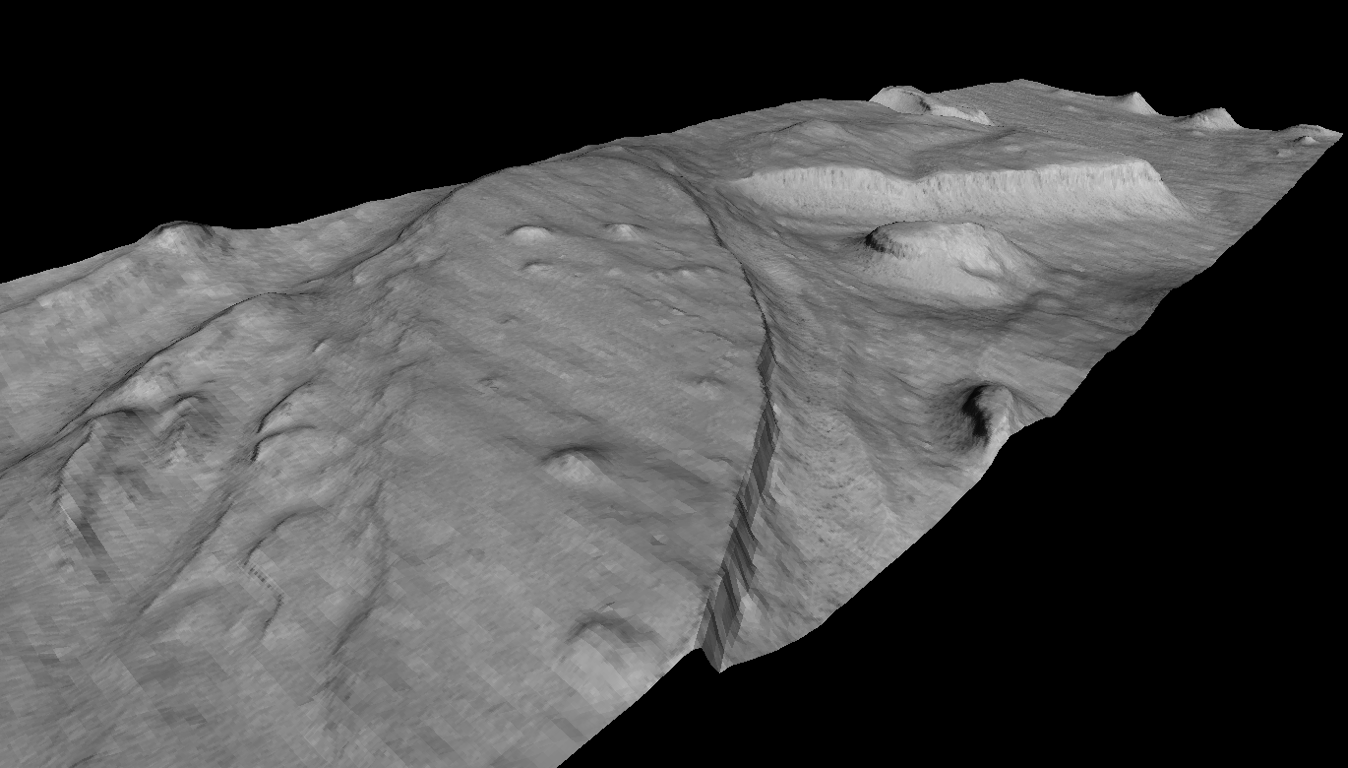
\includegraphics[width=6.5in]{images/introduction/p19view2.png} 
   \caption{This 3D model was generated from a \acf{MOC} image
     pair M01/00115 and E02/01461 (34.66N, 141.29E).  The complete
     stereo reconstruction process takes approximately thirty minutes on
     a 3.0~GHz workstation for input images of this size ($1024 \times 8064$
     pixels).  This model, shown here without vertical 
     exaggeration, is roughly 2~km wide in the cross-track
     dimension. }
   \label{fig:p19}
\end{figure}

\section{Background}

The \ac{IRG} at the NASA Ames Research Center has been developing
3D surface reconstruction and visualization capabilities for planetary
exploration for more than a decade.  First demonstrated during the
Mars Pathfinder Mission, the \ac{IRG} has delivered tools providing
these capabilities to the science operations teams of the Mars Polar
Lander (MPL) mission, the \ac{MER} mission, the \ac{MRO} mission,
and most recently the \ac{LRO} mission. A critical component
technology enabling this work is the \acf{ASP}.  The Stereo Pipeline
generates high quality, dense, texture-mapped 3D surface models
from stereo image pairs.

Although initially developed for ground control and scientific
visualization applications, the Stereo Pipeline has evolved in recent
years to address orbital stereogrammetry and cartographic
applications.  In particular, long-range mission planning requires
detailed knowledge of planetary topography, and high resolution
topography is often derived from stereo pairs captured from orbit.
Orbital mapping satellites are sent as precursors to planetary bodies
in advance of landers and rovers.  They return a wealth of imagery and
other data that helps mission planners and scientists identify areas
worthy of more detailed study. Topographic information often plays a
central role in this planning and analysis process.

Our recent development of the Stereo Pipeline coincides with a
period of time when \ac{NASA} orbital mapping missions are returning
orders of magnitude more data than ever before.  Data volumes from
the Mars and Lunar Reconnaissance Orbiter missions now measure in
the tens of Terabytes.  There is growing consensus that existing
processing techniques, which are still extremely human intensive
and expensive, are no longer adequate to address the data processing
needs of \ac{NASA} and the Planetary Science community.  To pick
an example of particular relevance, the \ac{HiRISE} Web site lists
1353 stereo pairs at the time of this writing \citep{HiRISE_website}.
Of these, only a few tens of stereo pairs have been processed to
date; mostly on human-operated, high-end photogrammetric workstations.
It is clear that much more value could be extracted from this
valuable raw data if a more streamlined, efficient process could be
developed.

The Stereo Pipeline was designed to address this very need.  By
applying recent advances in robotics and computer vision, we have
created an {\em automated} process that is capable of generating high
quality \acp{DEM} with minimal human intervention.  Users of the Stereo
Pipeline can expect to spend some time picking a handful of settings
when they first start processing a new type of imagery, but once this
is done the Stereo Pipeline can be used to process tens, hundreds, or
even thousands of stereo pairs without further adjustment.  With the
release of this software, we hope to encourage the adoption of this
tool chain at institutions that run and support these remote sensing
missions.  Over time, we hope to see this tool incorporated into
ground data processing systems alongside other automated image
processing pipelines.  As this tool continues to mature, we believe
that it will be capable of producing digital elevation models of
exceptional quality without any human intervention.

\section{Human vs. Computer: When to Choose Automation}

When is it appropriate to choose automated stereo mapping over the use
of a conventional, human-operated photogrammetric workstation?  This
is a philosophical question with an answer that is likely to evolve
over the coming years as automated data processing technologies become
more robust and widely adopted.  For now, our opinion is that you
should {\em always} rely on human-guided, manual data processing
techniques for producing mission critical data products for missions
where human lives or considerable capital resources are at risk.  In
particular, maps for landing site analysis and precision landing
absolutely require the benefit of an expert human operator to
eliminate obvious errors in the \ac{DEM}; and also to guarantee that the
proper procedures have been followed to correct satellite telemetry
errors so that the data have the best possible geodetic control.

When it comes to using \acp{DEM} for scientific analysis, both techniques
have their merits.  Human-guided stereo reconstruction produces \acp{DEM}
of unparalleled quality that benefit from the intuition and experience
of an expert.  The process of building and validating these \acp{DEM} is
well established and accepted in the scientific community. 

However, only a limited number of \acp{DEM} can be processed to this level
of quality.  For the rest, automated stereo processing can be used to
produce \acp{DEM} at a fraction of the cost.  The results are not
necessarily less accurate than those produced by the human operator,
but they will not benefit from the same level of scrutiny and quality
control.  As such, users of these \acp{DEM} must be able to identify
potential issues, and be on the lookout for errors that may result
from the improper use of these tools.  

We recommend that all users of the Stereo Pipeline take the time to
thoroughly read this documentation and build an understanding of how
stereo reconstruction and bundle adjustment can be best used together to
produce high quality results.  Please don't hesitate to contact us if
you have any questions!

\section{Software Foundations}

\subsection{NASA Vision Workbench}

The Stereo Pipeline is built upon the Vision Workbench software
which is a general purpose image processing and computer vision
library also developed by the \ac{IRG}.  Some of the tools discussed
in this document are actually Vision Workbench programs, but any
distribution of the Stereo Pipeline requires the Vision Workbench.
Unless you're compiling the Vision Workbench and Stereo Pipeline from
source, the distinctions probably won't matter to you.  


\subsection{The USGS Integrated Software for Imagers and Spectrometers}

This version of the Stereo Pipeline must be installed alongside a
compatible version of the \ac{USGS} \ac{ISIS}. \ac{ISIS} is widely
used in the planetary science community for processing raw spacecraft
imagery into high level data products of scientific interest such as
map projected and mosaicked imagery \cite{2004LPI....35.2039A,
  1997LPI....28..387G, ISIS_website}.  We chose \ac{ISIS} because (1)
it is widely adopted by the planetary science community, (2) it
contains the authoritative collection of geometric camera models for
planetary remote sensing instruments, and (3) it is open source
software that is easy to leverage.

By installing the Stereo Pipeline, you will be adding an advanced
stereo image processing capability that can be used in your existing
\ac{ISIS} work flow.  The Stereo Pipeline supports the \ac{ISIS}
``cube'' (\texttt{.cub}) file format, and can make use of the \ac{ISIS}
camera models and ancillary information (i.e. SPICE kernels) for
imagers on many \ac{NASA} spacecraft.  The use of this single standardized
set of camera models ensures consistency between products generated
in the Stereo Pipeline and those generated by \ac{ISIS}.  Also by
leveraging \ac{ISIS} camera models, the Stereo Pipeline can process
stereo pairs captured by just about any \ac{NASA} mission.

As an additional note, the Stereo Pipeline can also process arbitrary,
non-ISIS images with accompanying camera information, but doing so
requires a significant amount of extra work and setup.  This advanced
use of the software is not covered in this user's manual, however feel
free to contact us if you are interested in learning more about
adapting the pipeline to other stereo data sets.

%% It might be good to add a section on terminology someday...
%\section{Terminology}
%
%DISPARTY
%
%TRIANGULATION
%
%CORRELATION
%
%BUNDLE ADJUSTMENT

\pagebreak
\section{Getting Help}

All bugs, feature requests, and general discussion should be sent to
the Ames Stereo Pipeline user mailing list:
\begin{quote}
\indent \href{mailto:stereo-pipeline@lists.nasa.gov}{stereo-pipeline@lists.nasa.gov}
\end{quote}
To subscribe to this list, send an empty email message with the
subject `subscribe' (without the quotes) to:
\begin{quote}
\indent \href{mailto:stereo-pipeline-request@lists.nasa.gov}{stereo-pipeline-request@lists.nasa.gov}
\end{quote}
To contact the lead developers and project manager directly, send mail
to:
\begin{quote}
\indent \href{mailto:stereo-pipeline-owner@lists.nasa.gov}{stereo-pipeline-owner@lists.nasa.gov}
\end{quote}

\section{Typographical Conventions}

Names of programs that are meant to be run on the command line are
written in a constant-width font, like the \texttt{stereo} program,
as are options to those programs.

An indented line of constant-width text can be typed into your
terminal, these lines will either begin with a `\texttt{>}' to
denote a regular shell, or with `\texttt{ISIS}' which denotes an
\ac{ISIS}-enabled shell (which means you have set the \texttt{ISISROOT}
environment variable and sourced the appropriate \ac{ISIS} 3 Startup
script, as detailed in the \ac{ISIS} 3 instructions).
\begin{verbatim}
  > ls

  ISIS 3> pds2isis
\end{verbatim}

Italicized constant-width text denotes an option or argument that
a user will need to supply.  For example, `\texttt{stereo E0201461.map.cub
M0100115.map.cub out}' is specific, but `\texttt{stereo \textit{left-image
right-image} out}' indicates that \texttt{\textit{left-image}} and
\texttt{\textit{right-image}} are not the names of specific files,
but dummy parameters which need to be replaced with actual file
names.

Square brackets denote optional options or values to a command, and
items separated by a vertical bar are either aliases for each other, or
different, specific options.  Default arguments are prefixed by an equals
sign within parentheses, and line continuation with a backslash:

\texttt{  point2dem [--help|-h] [-r moon|mars] [-s \textit{float(=0)}] $\backslash$ } \\
\hspace*{6em}\texttt{[-o \textit{output-filename}] \textit{pointcloud}-PC.tif}

The above indicates a run of the \texttt{point2dem} program.  The
only argument that it requires is a point cloud file, which is
produced by the \texttt{stereo} program and ends in \texttt{-PC.tif},
although its prefix could be anything (hence the italics for that
part).  Everything else is in square brackets indicating that they
are optional.

Both \texttt{--help} and \texttt{-h} are really the same thing (both
will get you help).  Similarly, the argument to the \texttt{-r}
option must be either \texttt{moon} or \texttt{mars}.  The \texttt{-s}
option takes a floating point value as its argument, and has a
default value of zero.  The \texttt{-o} option takes a filename
that will be used as the output \ac{DEM}.

Although there are two lines of constant-width text, the backslash at the end
of the first line indicates that the command continues on the second line.  You 
can either type everything into one long line on your own terminal, or use the
backslash character (or appropriate line continuation character) and a return to 
continue typing on a second line in your terminal.


\section{Warnings to users of the Ames Stereo Pipeline ALPHA}

This is an {\bf ALPHA} release of the Stereo Pipeline.  There are many
known bugs and incomplete features. The API and command line options
will almost certainly change prior to the final release.  Some of the
documentation is incomplete and some of it may be out of date or
incorrect.  Although we hope you will find this release helpful, you
use it at your own risk.

While we are confident that the algorithms used by this software are
robust, they have not been systematically tested or rigorously
compared to other methods in the peer-reviewed literature. We have a
number of efforts underway to carefully compare Stereo
Pipeline-generated data products to those produced using established
processes, and we will publish those results as they become available.
In the meantime, {\bf we strongly recommend that you consult us first
  before publishing any results based on the cartographic products
  produced by this software}. You have been warned!

